% RESEARCH WORKING DRAFT -- not a submission-ready journal article.
% Visual form follows the TWO-COLUMN ELSEVIER 5p appearance of
% Chandra et al., arXiv:1811.08687 (published in EAAI).
% That paper is a design reference, NOT a Neural Networks journal template.
% Use pdfLaTeX + BibTeX on Overleaf; set this file as main.tex.
% For an actual journal submission, switch to the journal's CURRENT review
% template and anonymity rules. Do not present this course-scale dataset
% study as a completed multi-week journal extension.
\documentclass[final,5p,times,twocolumn]{elsarticle}
\usepackage{amsmath,amssymb}
\usepackage{graphicx}
\usepackage{booktabs}
\usepackage{array}
\usepackage{url}
\usepackage{microtype}
\usepackage[colorlinks=true,linkcolor=blue,citecolor=blue,urlcolor=blue]{hyperref}
\journal{Neural Networks}

\begin{document}
\begin{frontmatter}
\title{When Training Protocols Change the Winner: A Factorial Study of Recurrent Networks for Long-Horizon Forecasting}
% Confirm author order, full legal names and affiliations together before
% sharing this file externally or uploading to an anonymous review system.
\author[au]{Muhammed Nehan Poovan Kulathil}
\author[au]{Ahmed Nagi}
\address[au]{College of Engineering and Information Technology, Ajman University, Ajman, United Arab Emirates}

\begin{abstract}
Architectural comparisons of recurrent predictors often rely on one training recipe, although long-horizon errors depend on both recurrent-state optimization and the feedback presented during learning. We examine this dependency in a controlled, two-task study of vanilla recurrent neural networks (RNNs), long short-term memory networks (LSTMs), gated recurrent units (GRUs), and echo state networks (ESNs). On a simulated Mackey--Glass signal and a 321-customer aggregate of hourly electricity load, each predictor observes 100 samples and is evaluated through 100 autoregressive forecast steps. For RNNs, LSTMs, and GRUs we cross three truncated-backpropagation lengths, two gradient-clipping settings, three teacher-forcing policies, and three seeds, yielding 324 runs. A separate reservoir-size sweep contributes 18 ESN runs. An exploratory factorial analysis identifies architecture--teacher-forcing interactions in both tasks after within-task false-discovery-rate correction. The validation-selected ESN gives $0.0208\pm0.0075$ test normalized root-mean-square error (NRMSE) on Mackey--Glass, whereas the selected GRU gives $0.3318\pm0.0387$ on electricity. Four of nine electricity ESN runs also exhibit extreme but finite recursive errors, demonstrating why numerical completion does not imply forecast reliability. We report the mismatched ESN training objective and CPU fitting path explicitly, precluding an unqualified efficiency comparison. These findings support training-policy-aware evaluation rather than a universal architecture ranking; larger multi-dataset replication remains necessary before journal-level generalization.
\end{abstract}

\begin{keyword}
Recurrent neural networks \sep Teacher forcing \sep Truncated backpropagation through time \sep Echo state networks \sep Autoregressive forecasting \sep Experimental design
\end{keyword}
\end{frontmatter}

\section{Introduction}

A forecasting model trained to predict the next value in a sequence can fail when asked to predict the next hundred. The distinction is feedback. During training, an optimizer may supply the true previous observation; in a real forecast, the next input can be the model's own imperfect prediction. Small errors can then alter the subsequent hidden state and accumulate across a long open-loop rollout \cite{bengio2015scheduled,vlachas2024learning}. This mismatch complicates claims that one recurrent architecture is superior to another.

Other training decisions are similarly entangled with architecture. Truncated backpropagation through time (TBPTT) changes how far gradients propagate; gradient clipping modifies unusually large updates; and teacher forcing changes which inputs a network sees while its parameters are learned \cite{pascanu2013difficulty,aicher2020adaptively}. LSTM and GRU gates may moderate state dynamics differently from a vanilla RNN, while an ESN uses a fixed recurrent reservoir and fitted readout rather than gradient-based recurrent training \cite{hochreiter1997long,cho2014learning,lukosevicius2012practical}.

The core question is therefore not simply \emph{which recurrent model wins?} It is \emph{whether the model ranking changes with the training protocol and the data-generating process}. The distinction matters especially for chaotic or strongly periodic sequences, for which a locally plausible prediction need not remain plausible under repeated feedback. Existing studies cover gated-model comparisons, reservoir forecasting, gradient bias, and scheduled sampling individually \cite{greff2017lstm,shahi2022prediction,aicher2020adaptively,bengio2015scheduled}; our study brings several training choices into a single logged factorial comparison, without proposing a new neural architecture.

We examine four research questions: (RQ1) How does TBPTT length relate to 100-step error? (RQ2) Does clipping appreciably change recurrent-model outcomes at the tested budget? (RQ3) Do architecture and teacher-forcing policy interact, and does the favorable policy transfer between tasks? (RQ4) How do ESNs compare on forecast accuracy and failure behavior when their different fitting procedure is reported transparently?

The contributions are limited and concrete: a complete $324$-run gradient-trained factorial grid; a separately identified $18$-run ESN sweep; evaluation of both selected configurations and the full feedback-policy grid; and explicit documentation of catastrophic \emph{finite} ESN errors that a nonfinite-only failure check would miss. The evidence concerns two univariate tasks and should be read as a reproducible experimental case study, not a comprehensive benchmark of modern time-series forecasting.

\begin{figure*}[t]
\centering
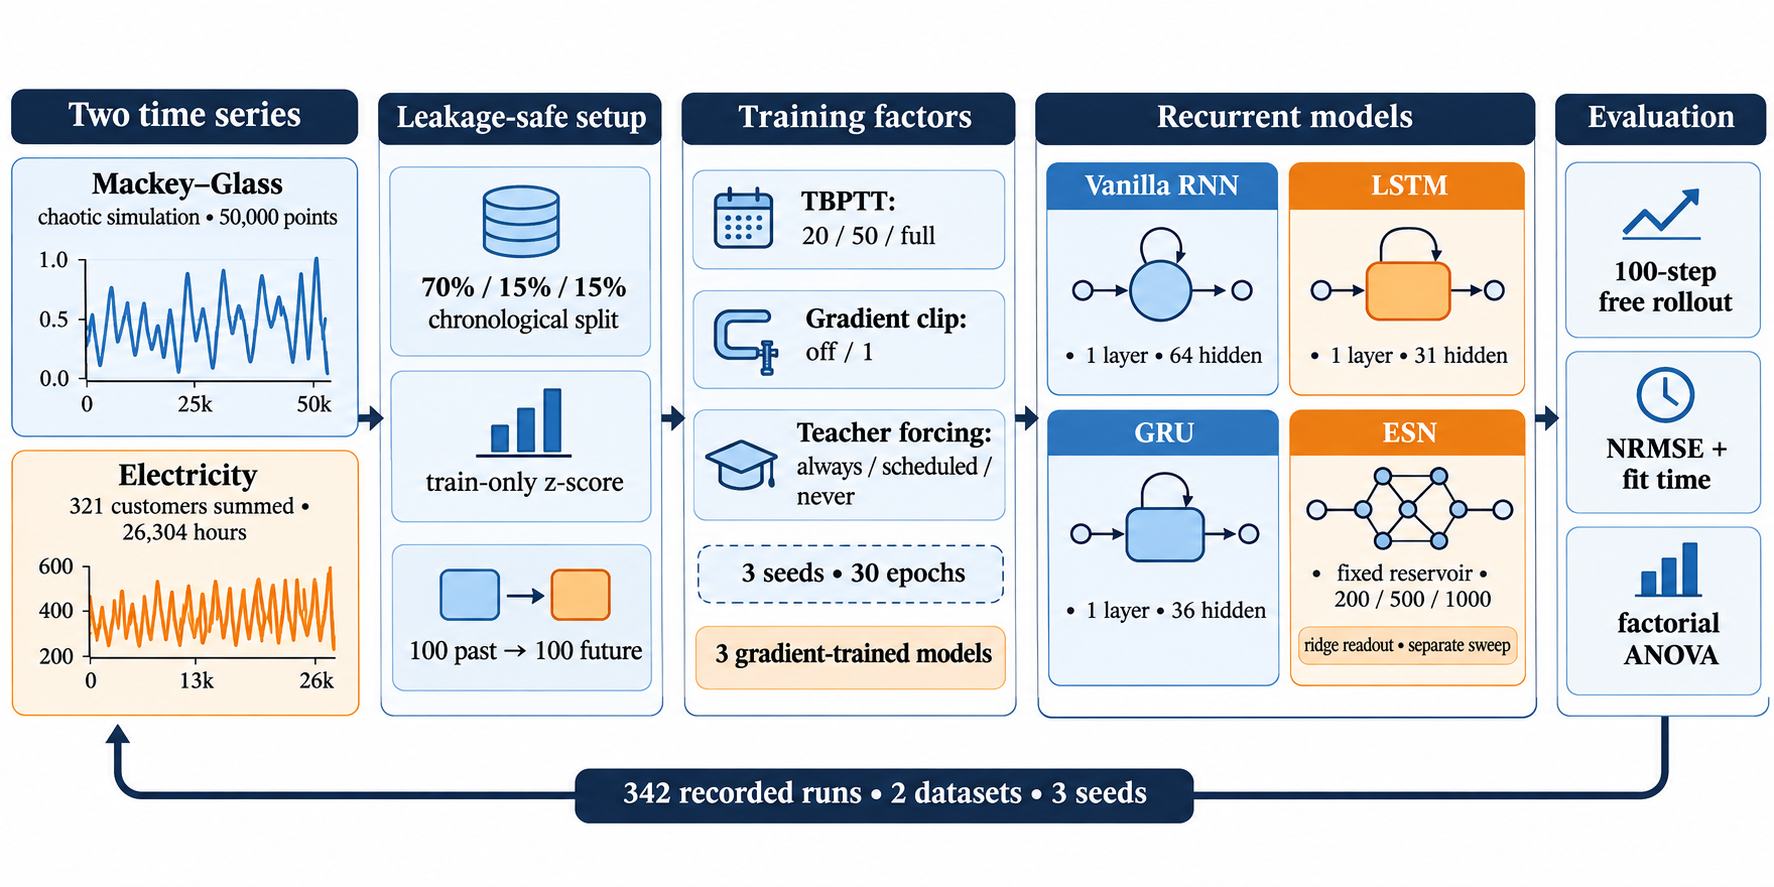
\includegraphics[width=\textwidth]{hero_pipeline_ai.png}
\caption{\textbf{Study overview.} Two univariate sequences are split chronologically, standardized using training-only statistics and converted to 100-context/100-target forecasting examples. Vanilla RNN, LSTM and GRU models are trained under a factorial grid of TBPTT, clipping and feedback conditions; an ESN is evaluated separately using fixed reservoirs and ridge-fitted readouts. All models are scored without future ground-truth feedback. The 342-run total comprises 324 gradient-trained runs and 18 ESN runs. \emph{Important:} the miniature signal traces and architecture icons are illustrative artwork, not measured data or gate-level diagrams. The ``three seeds/30 epochs'' training callout applies to the gradient-trained grid; ESN readouts are not trained for 30 epochs. This illustrative figure was created with OpenAI ImageGen in November 2026 from a research-configuration-specific prompt; the human authors must review it before publication. No diffusion model or U-Net was part of these forecasting experiments.}
\label{fig:pipeline}
\end{figure*}

\section{Background and Related Work}

\subsection{Recurrent models and memory}
For a scalar input $u_t$, a simple recurrent network updates a hidden state, schematically,
\begin{equation}
  h_t=\tanh(W_xu_t+W_hh_{t-1}+b),\qquad
  \hat{y}_t=w_o^\top h_t+b_o.
  \label{eq:rnn}
\end{equation}
The same state transition is repeatedly applied over time. An LSTM supplements this state with a cell state and input, forget, and output gates \cite{hochreiter1997long}; a GRU uses update and reset gates without a separate LSTM cell \cite{cho2014learning}. The gates provide learned pathways for retaining or replacing information, but their presence alone does not guarantee a better rollout. Prior empirical comparisons underscore that outcomes depend on task and training choices \cite{chung2014empirical,greff2017lstm,johnston2025revisiting}.

An ESN takes a different approach. A sparse recurrent reservoir is initialized and held fixed, while a regularized linear readout is estimated from its evolving states \cite{lukosevicius2012practical}. This can make fitting inexpensive for a given setup and has worked well in chaotic-series prediction \cite{shahi2022prediction}, but recurrent closed-loop behavior may be sensitive to reservoir parameters and readout amplification. The neural and ESN approaches therefore require both error metrics and a description of their unequal training workloads.

\subsection{Optimization horizon versus forecast horizon}
TBPTT limits the backward computational graph; the model can still process earlier observations forward in time. Truncation can reduce memory demands but biases gradients relative to full backpropagation \cite{aicher2020adaptively}. Clipping the gradient norm can prevent an unusually large update without solving the underlying temporal-credit-assignment problem \cite{pascanu2013difficulty}. Meanwhile, teacher forcing selects whether the next training input is the real observation or a generated prediction. Scheduled sampling interpolates between these behaviors \cite{bengio2015scheduled}. Work on prediction-conditioned learning and recurrent-state burn-in shows that these details remain scientifically active questions \cite{vlachas2024learning,schiller2026burnin}. Burn-in is cited here only as related work; it was \emph{not} varied in this study.

\section{Experimental Method}

\subsection{Two forecasting tasks}
\textbf{Mackey--Glass (MG).} The synthetic scalar series is generated from a classic delayed-feedback system \cite{mackey1977oscillation}:
\begin{equation}
 \frac{dx(t)}{dt}=\frac{0.2x(t-17)}{1+x(t-17)^{10}}-0.1x(t).
 \label{eq:mg}
\end{equation}
A forward-Euler integration uses a numerical step of $\Delta t=0.1$, but retains only every tenth update, giving one recorded observation per simulated time unit. We retain 50,000 observations after a 2,000-time-unit transient. This is a deterministic nonlinear experiment, not a sampled physical sensor stream; a 100-observation forecast horizon therefore covers 100 simulated time units.

\textbf{Electricity (ELEC).} The real-data task is derived from 321 hourly customer series in the Monash Time Series Forecasting Archive \cite{godahewa2021monash}. Customer values are summed at each timestamp to form one aggregate of 26,304 hourly observations. Missing values within each customer stream are forward-filled, with leading unavailable values set to zero before aggregation. This transformation defines a \emph{new univariate aggregate task}: its errors must not be compared directly with published per-customer forecasting benchmarks. Here the 100-step horizon is 100 hours.

\begin{figure*}[t]
\centering
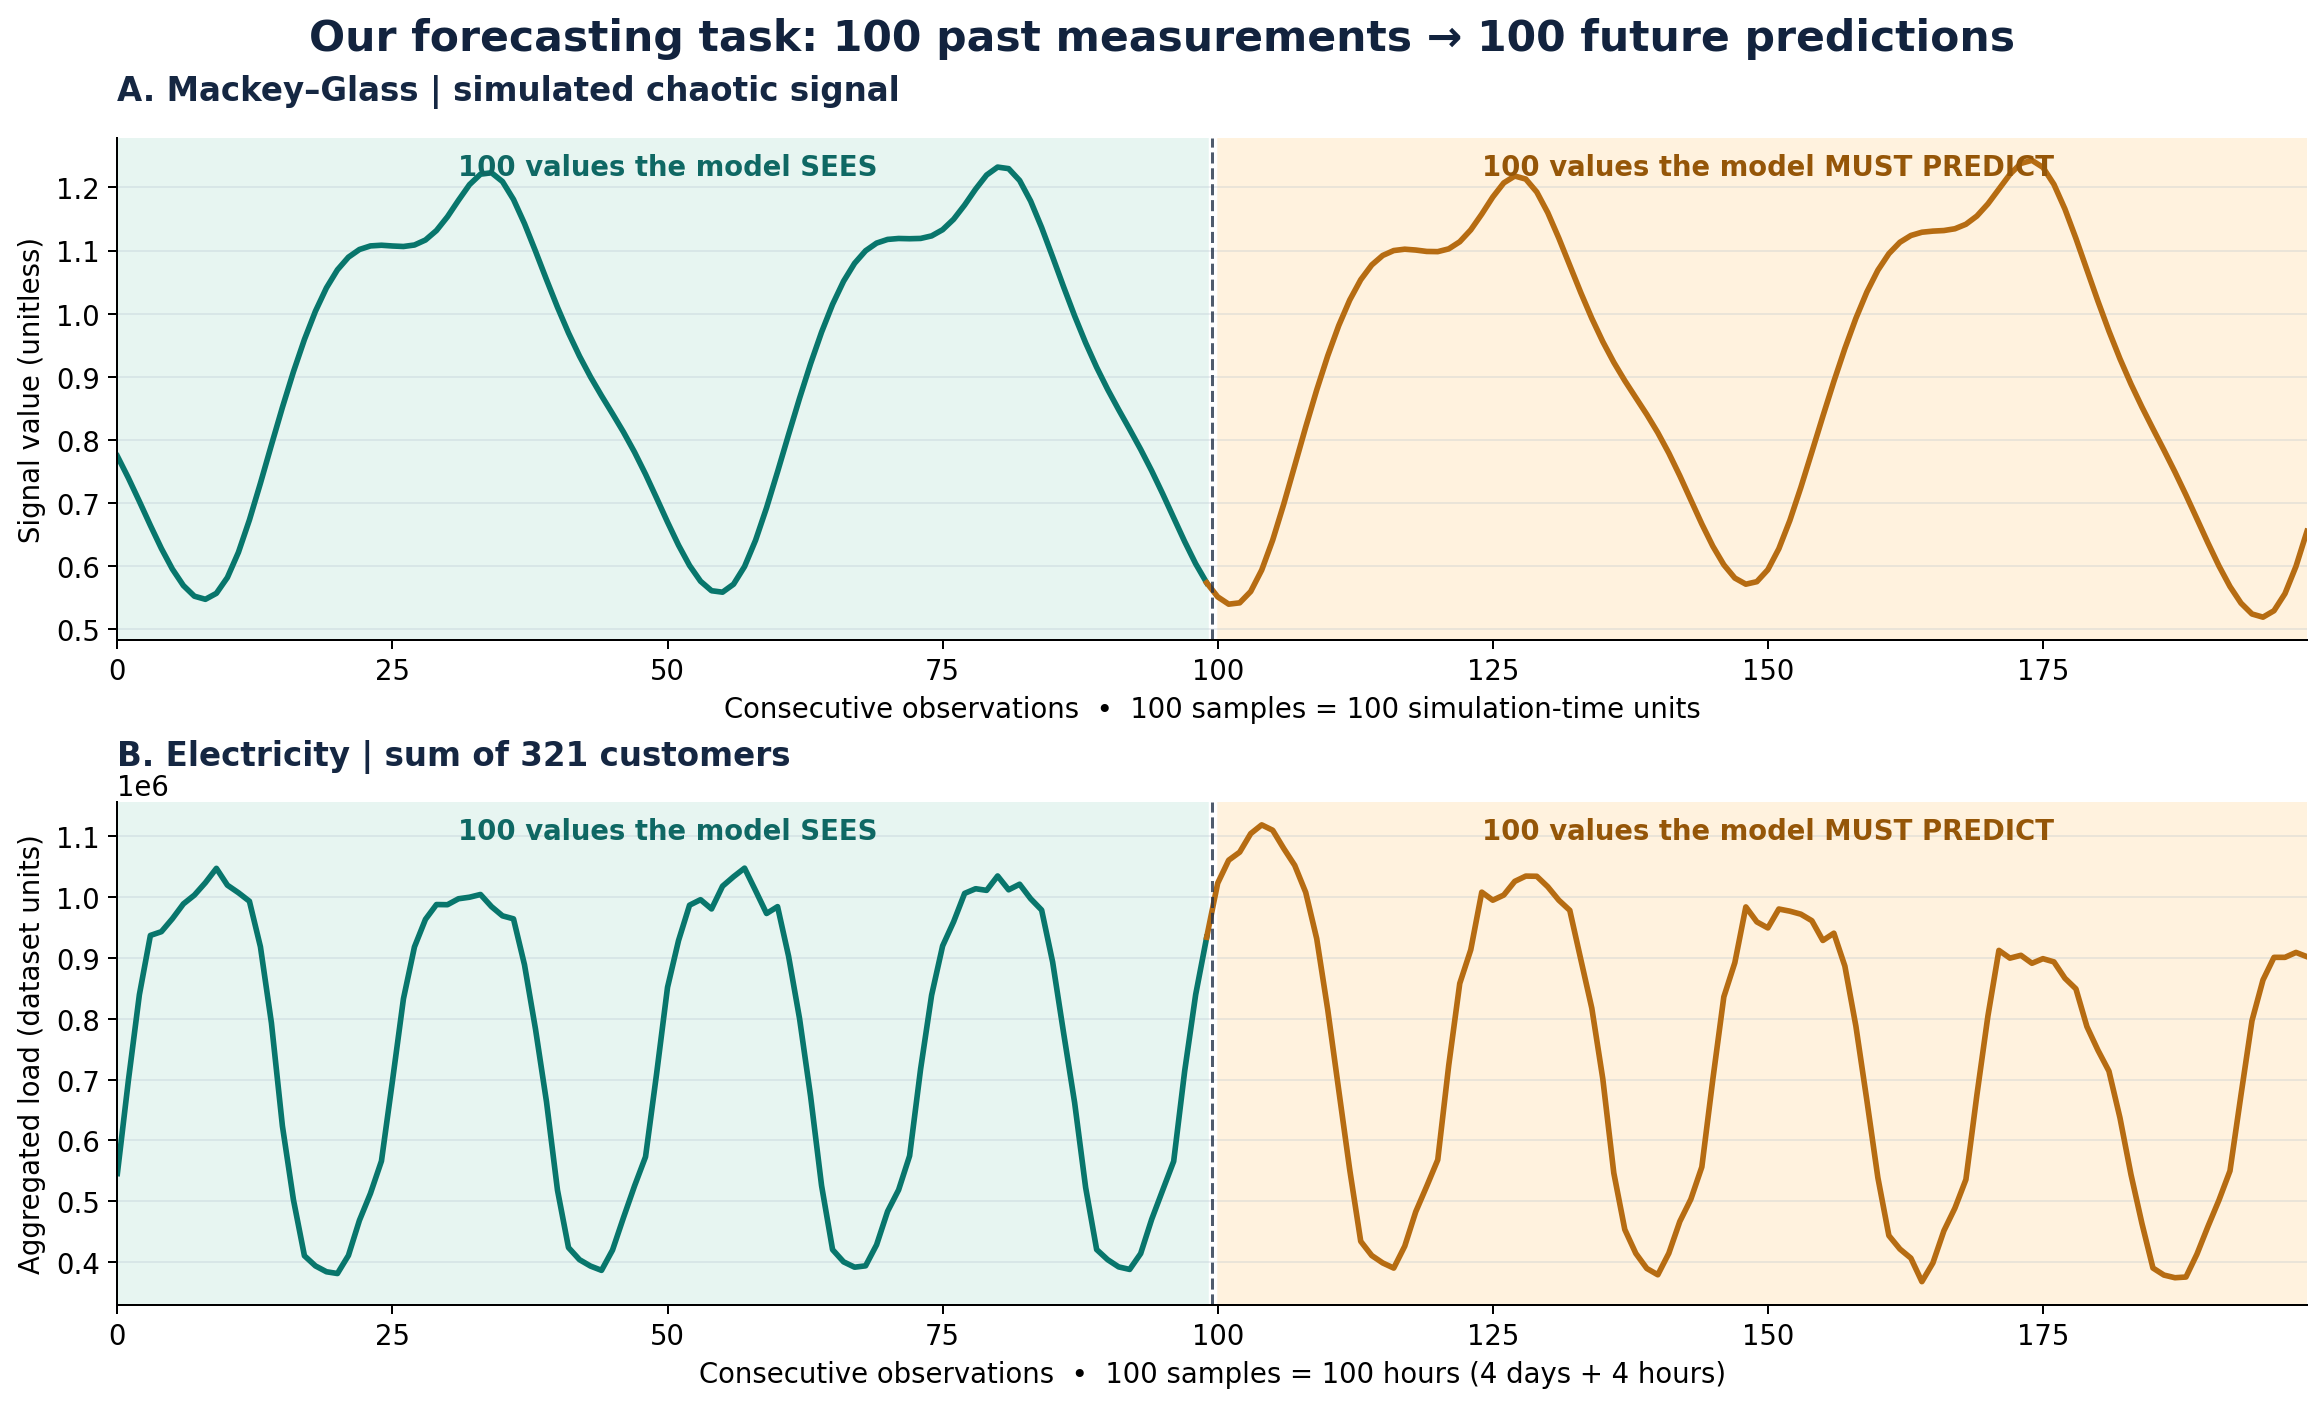
\includegraphics[width=.88\textwidth]{data_examples_measured.png}
\caption{Extracts of the \emph{actual saved series} and forecast-window examples used in the BAI301 experiment. Mackey--Glass displays irregular nonlinear oscillations; the electricity aggregate displays pronounced demand periodicity and level shifts. Unlike the small illustrative signal icons in Fig.~\ref{fig:pipeline}, the curves in this panel are derived from the archived numerical sequences. This panel is a data illustration, not a model prediction.}
\label{fig:realdata}
\end{figure*}

\begin{table}[t]
\caption{Task construction and held-out evaluation. Both tasks are univariate.}
\label{tab:datasets}
\centering
\footnotesize
\setlength{\tabcolsep}{4pt}
\begin{tabular}{p{.26\columnwidth}p{.26\columnwidth}p{.33\columnwidth}}
\toprule
Property & MG & Electricity \\
\midrule
Origin & Delayed chaotic simulation & Monash hourly aggregate \\
Series length & 50,000 & 26,304 \\
Granularity & 1 simulated time unit & 1 hour \\
Context / horizon & 100 / 100 & 100 / 100 \\
Test origins & at most 48 & 38 \\
Split order & \multicolumn{2}{l}{Chronological 70/15/15} \\
\bottomrule
\end{tabular}
\end{table}

\subsection{Chronological splits and rolling windows}
Each series is divided in temporal order into 70\% training, 15\% validation and 15\% test data. Standardization $z_t=(x_t-\mu_{\rm train})/\sigma_{\rm train}$ uses statistics computed \emph{only on the training portion}. A supervised instance contains past observations $(z_{t-99},\ldots,z_t)$ and 100 subsequent targets $(z_{t+1},\ldots,z_{t+100})$. We keep forecast windows inside the appropriate split, avoiding future leakage from validation or test observations into the training input.

Training-window origins are separated by stride 25 and uniformly subsampled to a cap of 512 origins; validation and test origins use stride 100 with a cap of 48. The electricity held-out portion provides 38 valid evaluation origins. These caps keep the grid feasible but limit how much of the available training data the gradient-trained models see. For scoring, a model may use the observed 100-value \emph{context}, but never the true future 100-value \emph{target} sequence as autoregressive feedback.

\subsection{Architectures and matched neural capacity}
We use single-layer RNN, LSTM and GRU predictors with scalar outputs, implemented in PyTorch \cite{paszke2019pytorch}. Their hidden widths are 64, 31, and 36; parameter counts are similar (4,353, 4,248, and 4,249 respectively), partly controlling model size while retaining the respective state-transition mechanisms. This is approximate parameter matching, not equality of representational capacity or floating-point operation count. Each model receives the same 100-value input context and is evaluated through recursive one-value-at-a-time prediction.

The ESN instead uses a fixed sparse recurrent reservoir of 200, 500 or 1,000 units, density 0.01, input scale 0.5, and a fitted ridge-regression readout. An illustrative leaky-reservoir update is
\begin{equation}
 r_t=(1-a)r_{t-1}+a\tanh(W_r r_{t-1}+W_{in}u_t),
 \label{eq:esn}
\end{equation}
where $a$ is the leak rate and recurrent weights are not optimized by backpropagation. The implementation performs a 100-step washout and considers five prespecified $(\rho,a,\lambda)$ triples for spectral-radius target, leak and ridge penalty. These are tuned at 200 reservoir units before the size sweep. The resulting ESN setup differs materially from the recurrent gradient-trained models.

\subsection{Factorial training protocols}
For the three trainable recurrent families, each run belongs to the complete grid in Table~\ref{tab:factors}. TBPTT is varied over 20, 50 or full recurrent steps; the full unrolled input sequence spans $100+100-1=199$ steps. At a truncation boundary, the relevant recurrent states and generated feedback are detached from the gradient graph. All truncation settings receive a single optimizer update per minibatch, rather than extra updates for shorter segments. Clipping, when enabled, constrains the global gradient norm to one.

\begin{table}[t]
\caption{Recorded experimental factors. The ESN sweep is separate.}
\label{tab:factors}
\centering
\footnotesize
\begin{tabular}{ll}
\toprule
Factor & Levels \\
\midrule
Task & MG; Electricity \\
Gradient-trained architecture & RNN; LSTM; GRU \\
TBPTT & 20; 50; full ($199$) \\
Gradient clipping & off; norm $1$ \\
Observed-target feedback & always; scheduled; never \\
Initialization seed & 42; 123; 2026 \\
\midrule
Gradient-trained runs & $2\times3\times3\times2\times3\times3=324$ \\
ESN reservoir units & 200; 500; 1000 \\
ESN runs & $2\times3\times3=18$ \\
\textbf{Total logged runs} & \textbf{342} \\
\bottomrule
\end{tabular}
\end{table}

\textbf{Always-observed feedback} supplies the real preceding value while constructing training-time predictions; \textbf{never-observed feedback} supplies the model's preceding prediction. Under \textbf{scheduled feedback}, the probability of using the real value in epoch $e\in\{0,\ldots,E-1\}$ is $p_e=\max(0,1-e/(E-1))$, with $E=30$. Each feedback decision is sampled independently from this probability in the recorded implementation. At evaluation \emph{every} configuration uses its own previous predictions as feedback. This makes all reported 100-step metrics comparable at the evaluation-protocol level even when their training conditions differ.

\begin{figure*}[t]
\centering
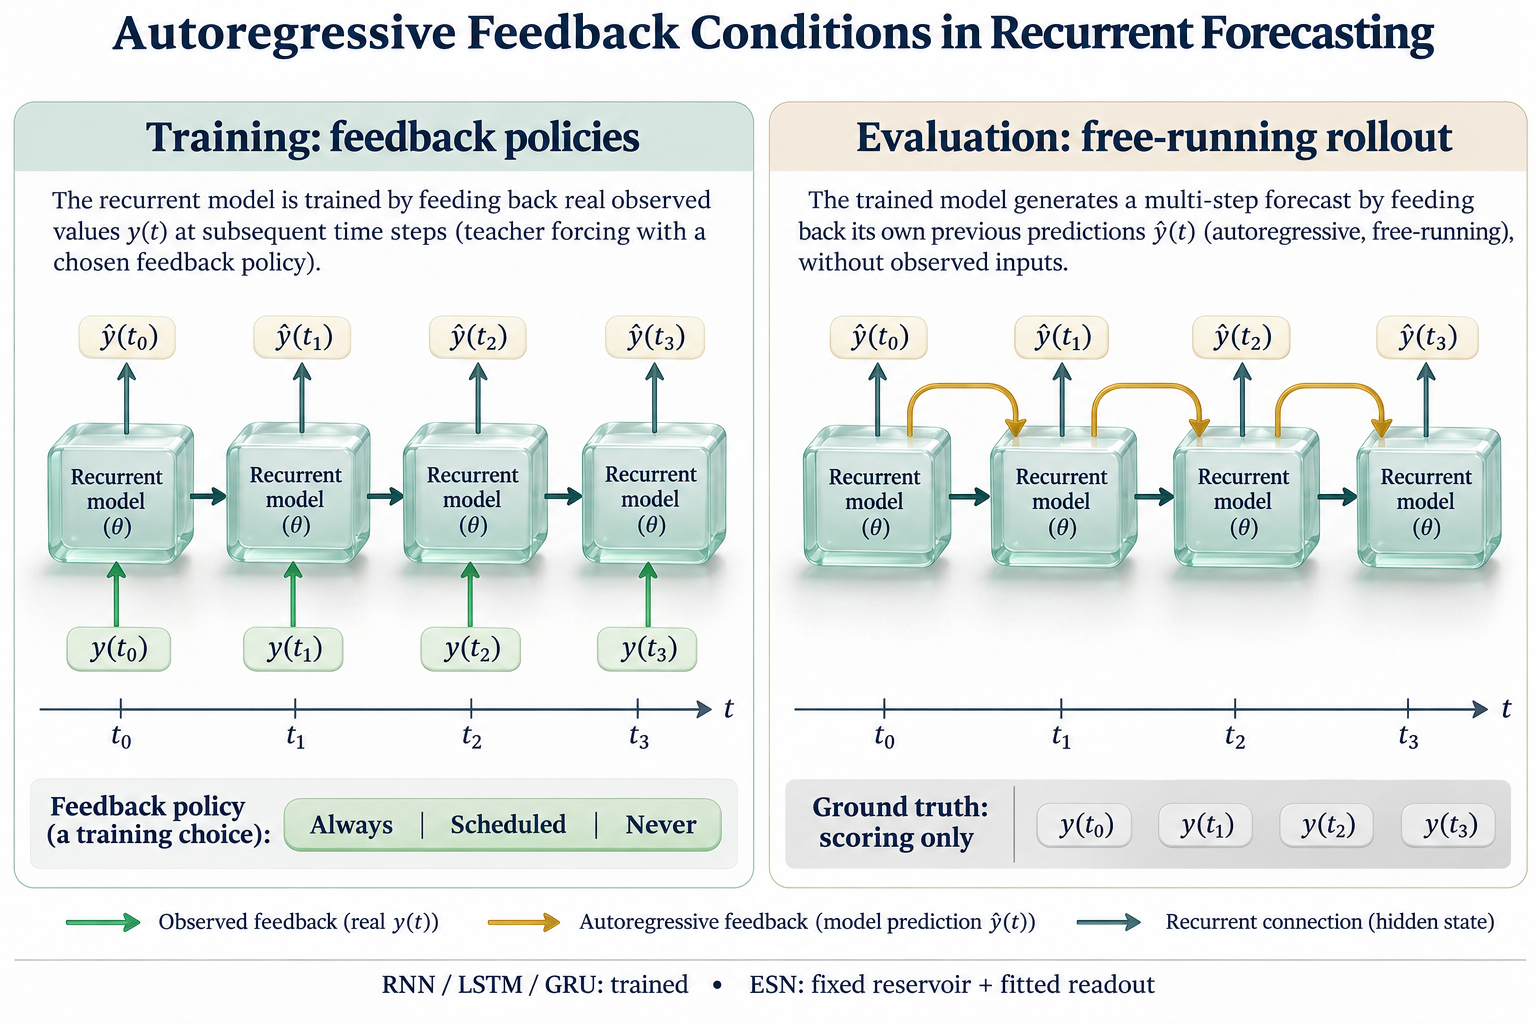
\includegraphics[width=.86\textwidth]{feedback_rollout_ai.png}
\caption{Conceptual difference between training feedback and free-running evaluation. The left panel sketches the fully teacher-forced case; scheduled and never-observed conditions substitute model predictions for some or all observed inputs. The right panel gives the actual test-time rule: previously generated predictions are fed back for subsequent steps, while true future samples are used only to score errors. This is explanatory OpenAI ImageGen artwork (November 2026), not a numerical experimental result or an exact unfolded computational graph.}
\label{fig:rollout}
\end{figure*}

The neural models are trained for 30 epochs with batch size 64. Before the main grid, a common learning-rate search over $\{10^{-4},3\times10^{-4},10^{-3},3\times10^{-3},10^{-2}\}$ uses 3 tuning epochs, 128 training origins and 12 validation origins for each architecture and dataset. Model checkpoints are assessed by validation recursive error at epochs 1, 10, 20 and 30. Configuration selection is based on validation results, not test results. ESN readouts are instead fitted by ridge regression on at most 6,000 states from the \emph{continuous} training series. This uses a different learning target and sample exposure than the 512-window neural optimization; we preserve this distinction when discussing speed.

\subsection{Forecasting metrics, runtime and inference}
Let $\widehat{Y}\in\mathbb{R}^{N\times H}$ be the test predictions and $Y$ the aligned true future values, with $H=100$. We report the pooled free-running normalized error
\begin{equation}
 \mathrm{NRMSE}=\frac{\left[\frac{1}{NH}\sum_{i=1}^{N}\sum_{h=1}^{H}(\widehat{Y}_{ih}-Y_{ih})^2\right]^{1/2}}{\sigma_{\mathrm{train}}}.
 \label{eq:nrmse}
\end{equation}
The denominator is the training-series standard deviation, not the test-series standard deviation; a lower NRMSE is better. We additionally log unnormalized error at horizons 1, 20, 50 and 100, fitting time, pre-clipping gradient statistics, and available memory measurements. For a simple contextual baseline, persistence repeats the final observed value for all future steps, $\widehat y_{t+h}=y_t$.

The neural processes ran in a Kaggle environment exposing two NVIDIA Tesla T4 GPUs, PyTorch 2.11.0 and CUDA 13.0. The gradient-trained memory measure is peak PyTorch-allocated GPU memory, \emph{not} whole-system peak consumption. The ESN uses a CPU linear-algebra path and its archived memory measure is process-level resident set size (RSS), which includes unrelated allocations. CPU RSS and allocated GPU memory cannot form a common memory-efficiency ranking. Likewise, ESN readout-fitting seconds and 30-epoch neural fitting seconds reflect different objectives and hardware paths, not a controlled speedup experiment.

The exploratory significance analysis fits a full four-factor ANOVA to $\log(1+\mathrm{NRMSE})$, includes seed as a blocking term, and tests main effects and interactions for the $324$ gradient-trained configurations only. The Benjamini--Hochberg false-discovery-rate adjustment is applied across 16 tested effects (including the seed block) \emph{within each task}. This analysis should be interpreted cautiously: evaluation windows from one series are correlated, multiple settings share seeds, and three seeds do not provide broad independent replication. We do not treat the ANOVA as causal identification of a universal architecture effect.

\section{Results}

\subsection{Validation-selected models}
Table~\ref{tab:results} reports held-out 100-step errors for the validation-selected configuration of each architecture, averaged over three seeds. The persistence baseline is a deterministic point of reference and requires no fitting time. The main neural conclusion is task dependence: selected RNN accuracy is strongest among gradient-trained models on MG, while GRU performs best among all reported model families on electricity. Selected ESN performance is striking on MG, but one should not extrapolate from one synthetic chaotic system to broad real-world superiority.

\begin{table*}[t]
\caption{Test performance of validation-selected configurations. Mean $\pm$ standard deviation across three seeds; the persistence baseline has a single deterministic score. Time means fitting/readout-estimation seconds. \emph{Do not rank CPU ESN fit seconds against GPU neural training seconds as matched computational efficiency.}}
\label{tab:results}
\centering
\small
\setlength{\tabcolsep}{7pt}
\begin{tabular}{lrrrr}
\toprule
& \multicolumn{2}{c}{Mackey--Glass} & \multicolumn{2}{c}{Electricity aggregate} \\
\cmidrule(lr){2-3}\cmidrule(lr){4-5}
Model & Test NRMSE $\downarrow$ & Fit time (s) & Test NRMSE $\downarrow$ & Fit time (s) \\
\midrule
Persistence & $1.2454$ & --- & $1.3842$ & --- \\
Vanilla RNN & $0.5209\pm0.0140$ & $24.40\pm0.14$ & $0.6196\pm0.0074$ & $27.72\pm0.34$ \\
LSTM & $0.5584\pm0.0576$ & $32.19\pm0.05$ & $1.0590\pm0.0153$ & $29.28\pm0.51$ \\
GRU & $0.5839\pm0.0413$ & $29.36\pm0.27$ & $\mathbf{0.3318\pm0.0387}$ & $28.08\pm0.26$ \\
ESN & $\mathbf{0.0208\pm0.0075}$ & $1.34\pm0.17$ & $0.7692\pm0.4292$ & $0.50\pm0.19$ \\
\bottomrule
\end{tabular}
\end{table*}

For MG, the ESN validation-selected reservoir size is 1,000 units; for electricity, it is 500 units. The comparison against persistence establishes that the selected RNN, LSTM, GRU and ESN each beat the simple last-value baseline on average for both tasks, but such an aggregate statement can conceal severe individual failures. The ESN worst-case behavior below is therefore a necessary complement to Table~\ref{tab:results}.

\begin{figure}[t]
\centering
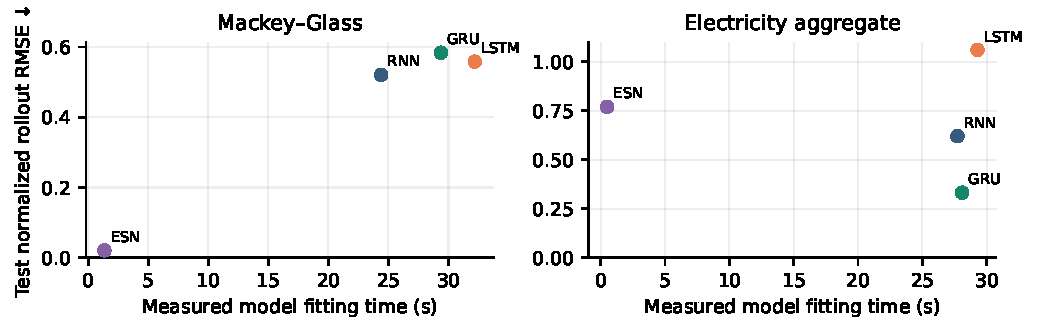
\includegraphics[width=\columnwidth]{accuracy_time.pdf}
\caption{Test NRMSE versus logged fitting seconds for validation-selected architectures on both tasks. This is a quantitative plot reconstructed from experiment records, not AI illustration. The ESN point corresponds to a different supervision objective and CPU fitting procedure; distances along the horizontal axis are descriptive only.}
\label{fig:accuracy}
\end{figure}

\subsection{Teacher forcing interacts with architecture}
The architecture--teacher-forcing interaction is present in the exploratory full factorial model for both MG ($F=7.05$, $p=4.54\times10^{-5}$; BH-adjusted $q=3.63\times10^{-4}$) and electricity ($F=17.92$, $p=2.87\times10^{-11}$; $q=2.30\times10^{-10}$). This is the most robust statistical pattern in the recorded grid, although the inference caveats above still apply. The global feedback-policy effect also survives BH correction for both signals. On electricity, the architecture main effect is pronounced ($q=6.02\times10^{-43}$), but on MG the main architecture effect among only RNN/LSTM/GRU is not significant ($p=0.181$) after pooling across the training policies.

\begin{table}[t]
\caption{Selected exploratory ANOVA outcomes for the gradient-trained grid. Adjusted $q$-values account for 16 within-task tested effects.}
\label{tab:anova}
\centering
\footnotesize
\setlength{\tabcolsep}{4pt}
\begin{tabular}{llrr}
\toprule
Task & Effect & Raw $p$ & BH $q$ \\
\midrule
MG & Architecture $\times$ forcing & $4.54\times10^{-5}$ & $3.63\times10^{-4}$ \\
ELEC & Architecture $\times$ forcing & $2.87\times10^{-11}$ & $2.30\times10^{-10}$ \\
MG & Architecture main & $0.181$ & not significant \\
MG & TBPTT main & $0.0127$ & not significant \\
\bottomrule
\end{tabular}
\end{table}

The interaction is not just a small shift in average. For the GRU, the median electricity NRMSE across the clipping/truncation/seed combinations is $0.349$ under always-observed training feedback and $0.629$ under never-observed training feedback. On MG the corresponding GRU medians reverse order: $0.955$ under always-observed versus $0.600$ under never-observed. These are descriptive medians over 18 runs per policy, not the validation-selected rows of Table~\ref{tab:results}. A global recommendation to always use, or never use, teacher forcing would ignore the task-dependent reversal.

\begin{figure}[t]
\centering
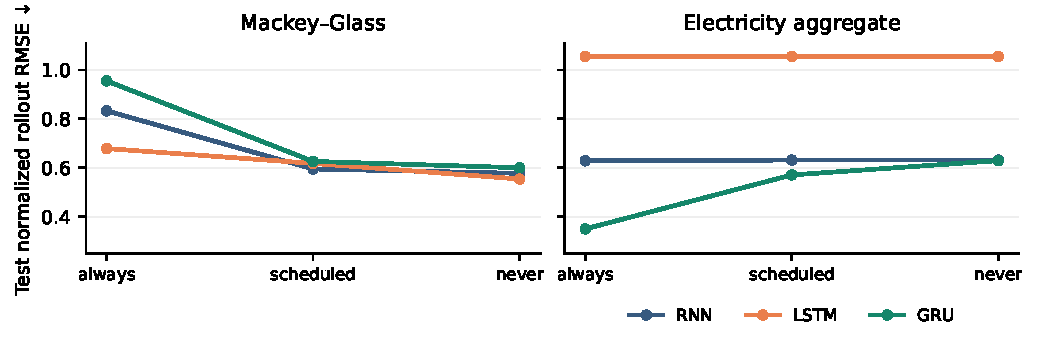
\includegraphics[width=\columnwidth]{forcing_interaction.pdf}
\caption{Median test NRMSE versus feedback choice for each gradient-trained architecture, combining truncation lengths, clipping states and three seeds (18 runs per point). The curves illustrate architecture--feedback interactions and differing behavior on MG and electricity. Results are descriptive; nominal significance is from the separate factorial model.}
\label{fig:interaction}
\end{figure}

The main clipping effect is not significant after BH correction in either task. The MG TBPTT main effect has raw $p=0.0127$, but it does not survive the multiple-test adjustment. We therefore cannot claim that clipping never helps or that a specific truncation length is optimal in general. The tested 30-epoch budget, small-capacity models and dataset-specific selection could suppress effects that emerge under another budget or task.

\subsection{One-step accuracy can mask long-rollout failure}
The selected electricity ESN has approximately $24.2\times10^3$ unnormalized one-step RMSE, compared with approximately $25.9\times10^3$ for the selected GRU. Yet over the full open-loop rollout their NRMSE scores are $0.769$ and $0.332$ respectively. This illustrates that similar early predictions do not guarantee similar closed-loop trajectories. Across only four architectures the ranking-agreement analysis is too small to support broad statistical conclusions (electricity Kendall's $\tau=0.333$, $p=0.75$).

\begin{figure}[t]
\centering
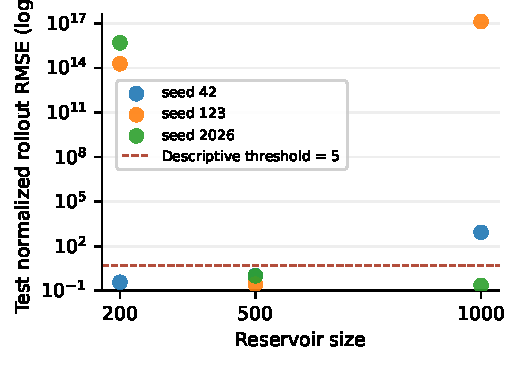
\includegraphics[width=\columnwidth]{electricity_esn_instability.pdf}
\caption{All nine electricity ESN runs, shown on a logarithmic NRMSE axis. Four exceed NRMSE $5$ while remaining numerically finite. Five is a \emph{post hoc descriptive threshold}, not a predefined success/failure criterion. The extreme points are included rather than suppressed.}
\label{fig:failure}
\end{figure}

Although all 342 runs completed and the experiment's finite-only checks reported no nonfinite forecasts, four of the nine electricity ESN runs recorded test NRMSE above five and the maximum was approximately $1.34\times10^{17}$. This severe instability is not visible from the validation-selected mean alone. The ESN's electricity tuning favored a spectral-radius target of $1.05$, which could contribute to amplified recursive feedback, but the current results do not isolate spectral radius causally; an explicit stability ablation is required. The apparent absence of ``failed runs'' therefore means absence of software/numerical exceptions under the logged criterion, \emph{not} absence of unreliable forecasts.

\subsection{Compute and memory interpretation}
The selected neural runs finish their training in about 24--32 seconds in the recorded GPU setting, while the selected ESN readout solves take roughly 0.5--1.3 seconds on the CPU path. These are \emph{not} end-to-end energy or matched-hardware measures. The selected neural runs report peak allocated GPU memory on the order of tens of MiB; the ESN's process RSS is roughly 6.5 GiB but includes host-process and environment allocations. Reporting either as a fair relative model-memory number would be misleading. We retain both logs as implementation diagnostics but do not assert an ESN speedup factor or a memory-efficiency winner.

\section{Discussion}

Three interpretations are supported. First, \emph{training protocol is part of the architecture comparison}: teacher-forcing policy changes outcomes differently for the three trainable recurrent families. Second, \emph{the type of series matters}: the simulated delay dynamics and aggregated hourly consumption represent different feedback challenges. Third, \emph{a single success metric is insufficient}: an ESN can be exceptionally good on one test and yield finite catastrophic rollouts under another setup. The right summary therefore includes seed variation, a horizon-long score, and explicit pathological runs.

There are also important results we do \emph{not} claim. We have not established a new architectural mechanism; a small $p$-value from this factorial design does not imply practical superiority on arbitrary datasets; near-matched parameter counts do not equalize compute; and ESN readout fitting is not experimentally matched to neural backpropagation. The excellent MG ESN performance is compatible with earlier reservoir-computing work \cite{shahi2022prediction}, not an unexpected state-of-the-art result. Contemporary work on recurrent gradients and burn-in also cautions against treating one recipe as definitive \cite{johnston2025revisiting,schiller2026burnin}.

\section{Threats to Validity and Journal-Extension Agenda}

\textbf{Data breadth.} Only one synthetic signal and one derived real-world aggregate are tested. Customer aggregation removes individual variability and masks domain-specific effects. Stronger generalization will require independent real-world series, a public benchmark protocol, and possibly multivariate tasks.

\textbf{Optimization budgets.} Gradient-trained networks share epoch counts, architecture-specific learning-rate tuning and a window cap, but no equal-compute or fully optimized Pareto frontier is established. ESNs use more continuous-state supervision and a separate CPU fit. Scaling to larger widths, longer budgets and matched prediction-target exposure could change rankings.

\textbf{Statistical independence.} The three seeds are not independent sampled datasets; overlapping and related test windows yield correlated errors. ANOVA residual assumptions are therefore uncertain, despite the reported BH correction. A stronger study should aggregate at independent series/episode level, use nested tuning, additional seeds, and hierarchical or paired uncertainty estimates.

\textbf{Reliability definition.} The experiment's automatic completion check tests finite execution, not bounded rollout error. Future experiments should prespecify failure thresholds, report prediction-magnitude distributions and coverage of unstable states, and control reservoir spectral radius, leak and output saturation.

\textbf{Research direction.} The most defensible multi-week extension is a targeted test of \emph{when feedback-policy choice is changed by TBPTT and recurrent-state burn-in}, motivated by recent burn-in research \cite{schiller2026burnin}. Replication across at least two additional real datasets, deliberately matched learning budgets, a predeclared analysis plan, and an ESN closed-loop stability sweep would constitute a materially stronger journal submission. These experiments are proposed, \emph{not} included in the present 342-run result set.

\section{Conclusion}
Under a shared 100-step free-running evaluation, 324 logged gradient-trained experiments reveal architecture--teacher-forcing interactions on both Mackey--Glass and aggregated electricity. Eighteen additional ESN runs demonstrate a complementary message: excellent accuracy on a chaotic simulation can coexist with severe finite closed-loop errors on real load. Our evidence favors careful experimental protocols and failure reporting over an unconditional claim that RNN, LSTM, GRU or ESN is ``best.'' The result is a reproducible starting point for a broader hypothesis-driven study, not yet a mature journal benchmark.

\section*{Data availability}
The Mackey--Glass experiment is reproducible from Eq.~\ref{eq:mg} and the documented integration, sampling and split parameters. The original electricity source is the Monash Time Series Forecasting Archive \cite{godahewa2021monash}. The accompanying reproducibility bundle includes the source generator, input-processing implementation, configuration, run-level CSV tables, individual run and epoch logs, and analysis code. Raw electricity data and its derived numeric sequence are omitted from the prospective public repository pending confirmation of redistribution terms; the code provides a source download path. A stable public repository URL must be inserted before submission.

\section*{Code availability}
An accompanying GitHub-ready source archive contains the executable Kaggle notebook, mechanically extracted training and analysis scripts, an environment requirements file, a documented short smoke test, and the full results tables and logs. Syntax checking and a CSV-level 342-run audit have been performed; independent execution of the full GPU experiment, a version-locked environment and an actual public hosted release remain outstanding. Do not state that a public repository exists until it has been verified.

\section*{Funding, competing interests and contributor roles}
The authors must confirm author order and contributions, institution affiliation, funding, conflicts, and acknowledgements before submission. This named working draft is \emph{not} formatted for a double-blind review process.

\section*{Declaration of generative AI and AI-assisted technologies in the manuscript preparation process}
During drafting, OpenAI ChatGPT was used to assist with language, structure and LaTeX organization. OpenAI ImageGen was used under author direction to produce the conceptual pipeline in Fig.~\ref{fig:pipeline} and training-feedback artwork in Fig.~\ref{fig:rollout} (November 2026; underlying generation-model identifier was not exposed). These images are illustrative; the dataset examples and all quantitative plots derive from saved numerical data. No diffusion model was trained or evaluated in this research. The human authors must critically verify every explanation, citation, figure, numerical result and declaration, revise the final manuscript as necessary, and assume responsibility for the paper's content.

\bibliographystyle{elsarticle-num}
\bibliography{references}

\end{document}
